%! TEX root = main.tex  % Specifies the main document file for multi-file projects

\chapter{SuperCollider as a Computer Music Language}

\section{Synth and SynthDef}

\subsection{Creating a SynthDef}

A SynthDef defines a new type of synthesizer in SuperCollider. The following example creates a simple SynthDef that outputs a sine wave:

\begin{supercollider*}
SynthDef.new("bee",
{ Out.ar(0, SinOsc.ar(440)) }
).add;
\end{supercollider*}

Explanation:

\begin{itemize}
    \item \texttt{SynthDef.new} creates a new SynthDef.
    \item \texttt{"bee"} is the name of this SynthDef.
    \item \texttt{Out.ar(0, SinOsc.ar(440))} sends the output of a sinusoidal oscillator to bus 0.
    \item \texttt{SinOsc.ar(440)} generates a sine wave at 440 Hz.
    \item \texttt{add} loads the SynthDef onto the server but does not save it to disk.
\end{itemize}

\begin{figure}[!htb]
    \centering
    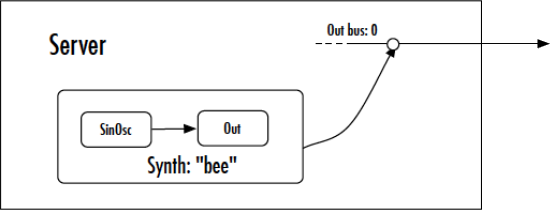
\includegraphics[width=0.7\linewidth]{00_Images/Res/04_chapter/01.png}
    \caption{bee SynthDef}
    \label{fig:beeSynthDef}
\end{figure}

\subsection{Signal Flow and UGen Graph}

Each SynthDef is represented as a UGen graph, which describes the relationships between unit generators and their parameters.

\subsection{SynthDef Arguments}

To allow parameter variation between different instances of a Synth, arguments can be added:

\begin{supercollider*}
SynthDef.new(\pulseSine, { arg out = 0, amp = 0.25, kfreq = 5;
    Out.ar(
        bus: out,
        channelsArray: SinOsc.ar(
            freq: kfreq * 50,
            mul: LFPulse.kr(freq: kfreq, width: 0.25)
        ) * amp
    );
}).add;
\end{supercollider*}

\begin{figure}[!htb]
    \centering
    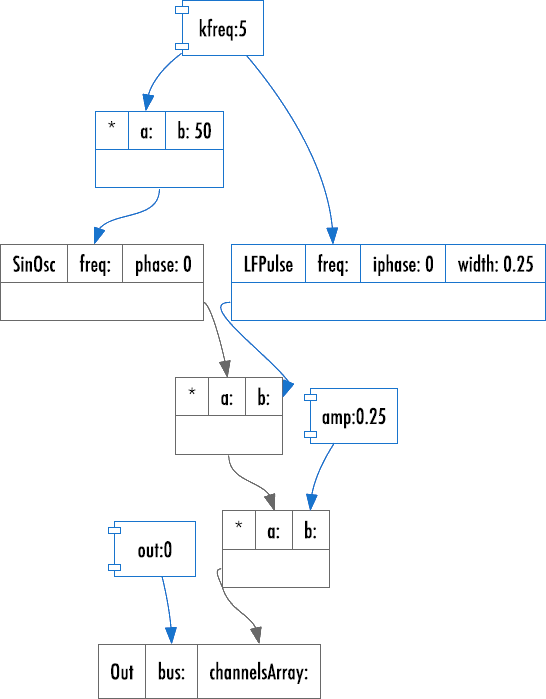
\includegraphics[width=0.6\linewidth]{00_Images/Res/04_chapter/02.png}
    \caption{SynthDef arguments}
    \label{fig:synthdefarguments}
\end{figure}

\subsection{Explanation of Arguments}

\begin{itemize}
    \item \texttt{arg out = 0, amp = 0.25, kfreq = 5;} declares default values for the arguments.
    \item \texttt{Out.ar(bus: out, channelsArray: ...)} assigns the output to the specified bus.
    \item \texttt{LFPulse.kr(freq: kfreq, width: 0.25)} generates a low-frequency pulse wave at control rate.
    \item The resulting Synth produces a sine wave that is periodically switched on and off based on the pulse wave.
\end{itemize}

\subsection{Creating a Synth from a SynthDef}

Once a SynthDef is defined, it can be instantiated as follows:

\begin{supercollider*}
c = Synth.new("pulseSine"); // Create and play the synth
d = Synth.newPaused(\pulseSine); // Create but do not play the synth
d.run(true); // Start the synth
d.run(false); // Pause the synth
d.set(\kfreq, 9); // Modify a parameter
d.free; // Deallocate the synth
\end{supercollider*}

\subsection{Mouse-Based Theremin}

This example maps mouse movement to control pitch and amplitude:

\begin{supercollider*}
SynthDef.new(\theremin, {
    Out.ar(0,
        SinOsc.ar(
            freq: MouseX.kr(200, 5000, 1),
            mul: MouseY.kr(0,1)
        )
    )
}).add;
\end{supercollider*}

Explanation:

\begin{itemize}
    \item \texttt{MouseX.kr(200, 5000, 1)} maps the horizontal mouse position to frequency.
    \item \texttt{MouseY.kr(0,1)} maps the vertical mouse position to amplitude.
\end{itemize}

\begin{figure}[!htb]
    \centering
    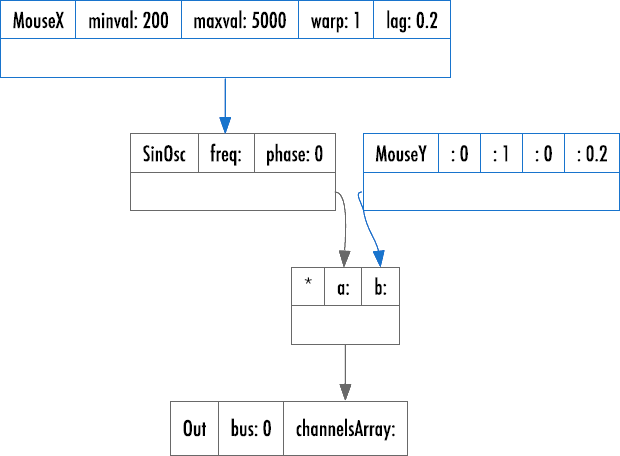
\includegraphics[width=0.55\linewidth]{00_Images/Res/04_chapter/03.png}
    \caption{Mouse-based theremin ugen graph}
    \label{fig:mouse-basedtheremin}
\end{figure}

\subsection{Implicit SynthDef}

SuperCollider allows playing a Synth without explicitly defining a SynthDef:

\begin{supercollider*}
{ SinOsc.ar(440, 0, 0.2) }.play;
\end{supercollider*}

When executed, a temporary SynthDef named \texttt{temp\_\_0} is automatically generated by SuperCollider. This method is useful for quick testing but inefficient for complex Synths.

\section{Controlling the Envelope of a Signal}

\subsection{Defining the Envelope Prototype}

SuperCollider allows controlling the temporal envelope of a signal using the \texttt{Env} class. The following example defines an envelope prototype:

\begin{supercollider*}
e = Env.new(
    levels:[0.0, 1.0, 0.5, 0.5, 0.0],
    times: [0.05, 0.1, 0.5, 0.35]
).plot;
\end{supercollider*}

This defines an ADSR-like envelope:

\begin{itemize}
    \item Attack lasts 0.05s, reaching a peak of 1.
    \item Decay lasts 0.1s, reducing the level to 0.5.
    \item Sustain lasts 0.5s at level 0.5.
    \item Release lasts 0.35s, fading to 0.
\end{itemize}

\begin{figure}[!htb]
    \centering
    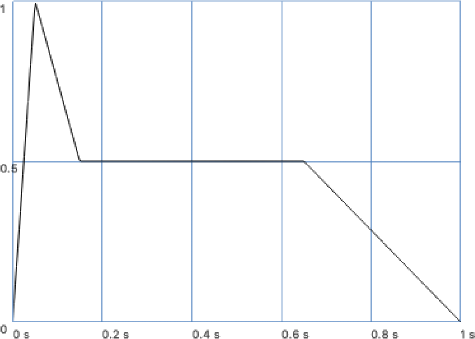
\includegraphics[width=0.7\linewidth]{00_Images/Res/04_chapter/04.png}
    \caption{Defining the envelope prototype}
    \label{fig:envelopeprototype}
\end{figure}

\subsection{Generating the Envelope with EnvGen}

The \texttt{EnvGen} class is used to apply the envelope to a signal at audio or control rate:

\begin{supercollider*}
EnvGen.ar(envelope, gate: 1, levelScale: 1, levelBias: 0, timeScale: 1, doneAction: 0)
EnvGen.kr(envelope, gate: 1, levelScale: 1, levelBias: 0, timeScale: 1, doneAction: 0)
\end{supercollider*}

Arguments:

\begin{itemize}
    \item \texttt{envelope}: An envelope created with \texttt{Env}.
    \item \texttt{gate}: Triggers the envelope each time the signal crosses zero in the positive direction.
    \item \texttt{levelScale}: Scales the amplitude.
    \item \texttt{levelBias}: Adds an offset to the amplitude.
    \item \texttt{timeScale}: Stretches (\textgreater1) or compresses (\textless1) the duration.
    \item \texttt{doneAction}: Defines the behavior at the end. \texttt{doneAction = 2} frees the synth, while \texttt{doneAction = 0} keeps it active.
\end{itemize}

\subsection{Examples of Envelope Application}

Using \texttt{EnvGen} to control amplitude:

\begin{supercollider*}
~env = Env.new(
    levels:[0.0, 1.0, 0.5, 0.5, 0.0],
    times: [0.05, 0.1, 0.5, 0.35]
);

{ SinOsc.ar(440) * EnvGen.kr(~env, 1, 1, 0, 1, 0) }.plot(2);
\end{supercollider*}

Modifying time and level scaling:

\begin{supercollider*}
{ SinOsc.ar(440) * EnvGen.kr(~env, 1, 2, 0, 2, 0) }.plot(2);
\end{supercollider*}

\subsection{Gating the Envelope}

The \texttt{gate} argument can be dynamically controlled. This example restarts the envelope every second using a low-frequency sine wave:

\begin{supercollider*}
~env = Env.new(
    levels:[0.0, 1.0, 0.5, 0.5, 0.0],
    times: [0.05, 0.1, 0.5, 0.35]
);

{ SinOsc.ar(440) * EnvGen.kr(~env, SinOsc.kr(1), 1, 0, 1, 0) }.plot(2);
\end{supercollider*}

\subsection{Predefined Envelope Types}

SuperCollider provides several built-in envelope types:

\begin{itemize}
    \item \texttt{Env.linen(atkT, sustT, relT, level, curve)}: Trapezoidal shape (no decay).
    \item \texttt{Env.triangle(dur, level)}: Triangular shape.
    \item \texttt{Env.sine(dur, level)}: Hanning window shape.
    \item \texttt{Env.perc(atkT, relT, level, curve)}: Typically percussive shape.
\end{itemize}

More envelope types can be found in the SuperCollider reference guide.

\section{Bus Management}

\subsection{Introduction to Busses}

Busses in SuperCollider are named after the analog mixing desk busses and are used to route signals between the audio hardware or different synths. There are two types of busses:

\begin{itemize}
    \item Audio rate busses, which transmit signals at the audio rate.
    \item Control rate busses, which transmit lower-frequency control signals.
\end{itemize}

\subsection{Bus Indexing}

Busses are accessed using numerical indices:

\begin{itemize}
    \item Control rate busses start from index \texttt{0}.
    \item Audio rate busses are indexed more complexly:
    
    \begin{itemize}
        \item The first \texttt{n} channels correspond to physical input and output busses, where:
        
        \begin{supercollider*}
        n = server.options.numOutputBusChannels + server.options.numInputBusChannels
        \end{supercollider*}
        
        \item Indices from \texttt{0} to \texttt{server.options.numOutputBusChannels -1} are hardware output busses.
        \item Indices from \texttt{server.options.numOutputBusChannels} onward are hardware input busses.
        \item The remaining indices are private busses for inter-synth communication.
    \end{itemize}
\end{itemize}

\subsection{Accessing Busses for Input and Output}

To write to an audio rate bus, use \texttt{Out.ar}:

\begin{supercollider*}
Out.ar(out, channelsArray);
\end{supercollider*}

\begin{itemize}
    \item \texttt{out} is the index of the target bus.
    \item \texttt{channelsArray} is the signal to be routed. If multichannel, the channels are mapped to consecutive busses.
\end{itemize}

To read from an audio rate bus, use \texttt{In.ar}:

\begin{supercollider*}
In.ar(bus: 0, numChannels: 1);
\end{supercollider*}

\begin{itemize}
    \item \texttt{bus} is the index of the first bus to read from.
    \item \texttt{numChannels} specifies how many consecutive busses to read.
\end{itemize}

Similar methods exist for control rate busses: \texttt{In.kr} and \texttt{Out.kr}.

\subsection{Example: Mixing Signals on the Same Bus}

When multiple synths write to the same bus, their outputs are mixed:

\begin{supercollider*}
(
SynthDef(\sine_mix, { arg freq = 440, out = 0;
    Out.ar(out, SinOsc.ar(freq, 0, 0.2));
}).send(s);
)

// Both synths write to bus 1, and their outputs are mixed
x = Synth(\sine_mix, ["out", 1, "freq", 660]);
y = Synth(\sine_mix, ["out", 1, "freq", 770]);
\end{supercollider*}

\subsection{Allocating Busses}

Busses can be allocated dynamically using the \texttt{Bus} class:

\begin{supercollider*}
// Allocate a 2-channel control bus
b = Bus.control(s, 2);

// Allocate a private audio bus
c = Bus.audio(s);
\end{supercollider*}

To read and write from these busses, use \texttt{Out.kr}, \texttt{Out.ar}, \texttt{In.kr}, and \texttt{In.ar}.

\subsection{Working with Busses}

\begin{supercollider*}
b = Bus.control(s, 2); // Create a 2-channel control bus
b.index; // Get the bus index
b.numChannels; // Get the number of channels

b.free; // Free the allocated bus
\end{supercollider*}

\subsection{Example: Using Busses to Control Frequency}

\begin{supercollider*}
(
SynthDef("tutorial-Infreq", { arg bus, freqOffset = 0;
    Out.ar(0, SinOsc.ar(In.kr(bus) + freqOffset, 0, 0.5));
}).send(s);

SynthDef("tutorial-Outfreq", { arg freq = 400, bus;
    Out.kr(bus, SinOsc.kr(1, 0, freq/40, freq));
}).send(s);

b = Bus.control(s, 1);
)

// Assign synths to bus
x = Synth.new("tutorial-Outfreq", [\bus, b]);
y = Synth.after(x, "tutorial-Infreq", [\bus, b]);
z = Synth.after(x, "tutorial-Infreq", [\bus, b, \freqOffset, 200]);

// Free resources
x.free; y.free; z.free; b.free;
\end{supercollider*}

\subsection{Execution Order Control with after}

\begin{itemize}
    \item Both \texttt{y} and \texttt{z} read from the same control bus \texttt{b}.
    \item \texttt{z} adds an offset of 200 Hz to the frequency.
    \item The \texttt{after} method ensures \texttt{y} and \texttt{z} are executed after \texttt{x}.
\end{itemize}

\section{Groups and Order of Execution}

\subsection{Groups}

In SuperCollider, synths on the server are classified as nodes. Another type of node is a group, which is a collection of nodes that can include both synths and other groups. Groups are useful for:

\begin{itemize}
    \item Controlling the order of execution of synths.
    \item Grouping nodes together to send messages collectively.
\end{itemize}

SuperCollider provides an abstraction object called \texttt{Group} to manage groups in the client application.

\subsection{Controlling the Order of Execution}

Busses facilitate communication between synths, but proper execution order must be maintained. If one synth writes to a bus and another reads from it, the latter must execute afterward to avoid outdated signals.

SuperCollider provides two arguments in \texttt{Synth.new} to control execution placement:

\begin{itemize}
    \item \texttt{target}: The group or synth that determines the execution order.
    \item \texttt{addAction}: Specifies the position of the new synth relative to the target.
\end{itemize}

If no target is provided, the synth is placed in the default group.

\begin{figure}[!htb]
    \centering
    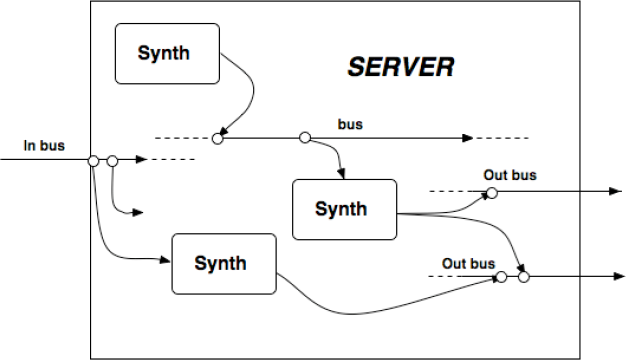
\includegraphics[width=0.7\linewidth]{00_Images/Res/04_chapter/08.png}
    \caption{Controlling the order of execution}
    \label{fig:controllingorder}
\end{figure}

\subsection{Synth Placement Methods}

SuperCollider provides several methods for precise placement of synths:

\begin{supercollider*}
Synth.new(defName, args, target, addAction);
\end{supercollider*}

\begin{itemize}
    \item If \texttt{target} is a synth, \texttt{addToHead} and \texttt{addToTail} place the synth at the beginning or end of the group.
    \item If \texttt{target} is a server, the synth is placed in the server's default group.
    \item If \texttt{target} is \texttt{nil}, it defaults to the main group of the default server.
\end{itemize}

Additional methods:

\begin{supercollider*}
Synth.head(aGroup, defName, args);
\end{supercollider*}

Places the new synth at the head of \texttt{aGroup}.

\begin{supercollider*}
Synth.tail(aGroup, defName, args);
\end{supercollider*}

Places the new synth at the tail of \texttt{aGroup}.

\begin{supercollider*}
Synth.before(aNode, defName, args);
\end{supercollider*}

Adds the new synth just before \texttt{aNode}.

\begin{supercollider*}
Synth.after(aNode, defName, args);
\end{supercollider*}

Adds the new synth just after \texttt{aNode}.

\begin{supercollider*}
Synth.replace(synthToReplace, defName, args);
\end{supercollider*}

Replaces \texttt{synthToReplace} with the new synth and frees the original node.

\subsection{Creating and Managing Groups}

Like synths, groups accept \texttt{target} and \texttt{addAction} arguments for controlled placement.

Example:

\begin{supercollider*}
g = Group.new;        // Create a new group
h = Group.before(g);  // Create a group before g
g.free;              // Free group g
h.free;              // Free group h
\end{supercollider*}

\section{Scheduling Events in SuperCollider}

\subsection{The Problem of Scheduling}

According to Edgar Varèse, music is "organized sound." This implies that musical composition involves two aspects:

\begin{itemize}
    \item Internal organization of sound, such as harmonic content and timbre.
    \item Temporal organization of events, which requires scheduling.
\end{itemize}

SuperCollider provides several methods to manage event scheduling.

\subsection{Scheduling through Pulse Generation}

A sequence of discrete events can be generated using pulse signals.

\begin{supercollider*}
SynthDef.new("pulseEvent", { |seqFreq = 4, sawFreq = 0.125, sinFreq = 0.14| 
    Out.ar(0,
        Pulse.kr(seqFreq, width:0.1, mul:0.5, add:0.5) *
        Formant.ar(
            fundfreq: (LFSaw.kr(sawFreq, mul:6, add:60) + SinOsc.ar(sinFreq, mul:3)).round.midicps
        )
    )
}).add; 

x = Synth.new("pulseEvent", [\seqFreq , 4]);
\end{supercollider*}

\subsection{Pulse and Formant UGens}

\texttt{Pulse.kr(freq, width, mul, add)} generates a band-limited pulse wave:

\begin{itemize}
    \item \texttt{freq}: Pulse frequency in Hz.
    \item \texttt{width}: Pulse width ratio (0.5 produces a square wave).
    \item \texttt{mul}, \texttt{add}: Scaling and offset parameters.
\end{itemize}

\texttt{Formant.ar(fundFreq, formFreq, bwFreq)} generates harmonic signals by filtering harmonics at \texttt{fundFreq}.

\subsection{Scheduling through Envelopes}

Envelopes can be used to create discrete events over time.

\begin{supercollider*}
(
{
    var freq = 422, cycleDur = 2;
    var env = Env([0,1,1,0,0,1,1,0, 0], [0,1,0, 1, 0, 2.5, 0, 1.5]);
    EnvGen.kr(env, 1, gate: Impulse.kr(1/cycleDur), timeScale: 1/5, doneAction: 0) 
    * SinOsc.ar(freq)
}.play
)
\end{supercollider*}

\subsection{Scheduling through Select}

\texttt{Select.kr(which, array)} chooses elements from an array based on an index.

\begin{supercollider*}
SynthDef(\select, {
    var array = Array.fill(64, {|i| (i%4) + (i%7) + (i%11) + 60});
    array = array.add(90).postln.midicps;
    Out.ar(0, Saw.ar(Select.kr(LFSaw.kr(1/6).linlin(-1.0,1.0, 0, array.size).round, array), 0.2));
}).add;

Synth(\select);
\end{supercollider*}

\subsection{Scheduling through the Demand UGen}

\texttt{Demand.kr(trig, reset, [..ugens..])} is triggered when \texttt{trig} becomes true.

\begin{supercollider*}
(
{
    var a, freq, trig;
    a = Dseq([1, 3, 2, 7, 8] + 60, 3);
    trig = Impulse.kr(4);
    freq = Demand.kr(trig, 0, a.midicps);
    Mix.fill(10, { Pulse.ar(freq + 5.rand) }) * 0.1;
}.play;
)
\end{supercollider*}

\subsection{Scheduling through Routine and Clocks}

SuperCollider provides different clocks for event scheduling:

\begin{itemize}
    \item \texttt{SystemClock}: High-priority clock, non-musical timing.
    \item \texttt{TempoClock}: Musical timing, default 60 BPM.
    \item \texttt{AppClock}: Low-priority, used for GUI activities.
\end{itemize}

Example of scheduling with \texttt{SystemClock}:

\begin{supercollider*}
(
"waiting for three seconds".postln;
SystemClock.sched(3.0, { "done".postln });
)
\end{supercollider*}

Example of using \texttt{Routine}:

\begin{supercollider*}
r = Routine.new({
    var time;
    10.do({ |i| 
        "slowing".postln;
        time = (i * 0.1).postln;
        time.wait;
    });
    1.wait;
    "the".postln;
    1.wait;
    "end".postln;
});
SystemClock.play(r);
\end{supercollider*}

\subsection{Using Fork for Scheduling}

Instead of explicitly defining a routine, the \texttt{fork} method schedules a function:

\begin{supercollider*}
(
{
    var amp = 0.125;
    var firstBit = Array.fill(32, {[0,1].choose});
    var secondBit = Array.fill(16, {[0,1].choose});
    var freq;

    firstBit.do{|i|
        freq = [2000, 2500][i];
        { SinOsc.ar(freq, mul: amp) * Line.kr(1,1,0.30, doneAction:2) }.play;
        0.03.wait;
    };

    0.04.wait;

    secondBit.do{|i|
        freq = [2000, 2500][i];
        { SinOsc.ar(freq, mul: amp) * Line.kr(1,1,0.30, doneAction:2) }.play;
        0.03.wait;
    };

    0.52.wait;

    { SinOsc.ar(1000, mul: amp) * LFPulse.ar(1, width:0.1) * Line.kr(1,1,5, doneAction:2) }.play;
    6.wait;
    { SinOsc.ar(1000, mul: amp) * Line.ar(1,1,0.1, doneAction:2) }.play;
}.fork;
)
\end{supercollider*}

\subsection{Scheduling with Patterns}

\texttt{Pseq} describes sequences by repeating a seed sequence.

\begin{supercollider*}
p = Pseq([1,2,3,4], 3).asStream;
13.do{ "next...? -> ".post; p.next.postln };
\end{supercollider*}

Example of using \texttt{Pseq} in a synth:

\begin{supercollider*}
SynthDef(\sinPerc, { |freq = 440, pos = 0, level = 0.125, detune = 0.025|
    var sig = Mix.fill(10, { SinOsc.ar(freq + Rand(0, freq * detune)) });
    sig = FreeVerb.ar(sig * EnvGen.kr(Env.perc));
    DetectSilence.ar(sig, -96.dbamp, doneAction:2);
    Out.ar(0, Pan2.ar(sig, pos, level));
}).add;

(
p = Pseq([0,2,4,3,10,13,12,6,5,7], inf).asStream;
{
    inf.do{
        Synth(\sinPerc, [\freq, (p.next+70).midicps]);
        0.25.wait;
    }
}.fork;
)
\end{supercollider*}

\section{Buffers}

\subsection{Introduction to Buffers}

A buffer is a memory space allocated to store data, typically used for audio storage and manipulation. Buffers in SuperCollider function similarly to busses but are used for sampled data instead of signal routing.

\subsection{Creating and Using Buffers}

A buffer can be allocated using:

\begin{supercollider*}
Buffer.alloc(server, numFrames, numChannels: 1, completionMessage, bufnum)
\end{supercollider*}

Example:

\begin{supercollider*}
(
var buf = Buffer.alloc(s, 2.pow(10));

// Fill buffer with a sine wave
buf.sine1([1]);

// Play the buffer using an oscillator
{Osc.ar(buf, 440)}.play;
)
\end{supercollider*}

\subsection{Buffer Methods}

\texttt{sine1(amps,norm: true,asWavetable: true,clearFirst: true)} fills the\hfill\\buffer with harmonics.

\begin{itemize}
    \item \texttt{amps}: Array of harmonic amplitudes.
    \item \texttt{norm}: Normalizes buffer peak to 1.0 (default: true).
    \item \texttt{asWavetable}: Stores as a wavetable for interpolation (default: true).
    \item \texttt{clearFirst}: Clears the buffer before writing (default: true).
\end{itemize}

For arbitrary phase relationships, use \texttt{sine3}.

\subsection{Oscillator Using Buffers}

The \texttt{Osc} class provides a wavetable lookup oscillator:

\begin{supercollider*}
Osc.ar(bufnum, freq: 440, phase: 0, mul: 1, add: 0)
\end{supercollider*}

\begin{itemize}
    \item \texttt{bufnum}: Buffer variable.
    \item \texttt{freq}: Frequency in Hz.
    \item \texttt{phase}: Phase offset in radians.
    \item \texttt{mul}, \texttt{add}: Scaling and offset parameters.
\end{itemize}

\subsection{Writing and Reading Audio Files}

\paragraph{Writing a File}

The \texttt{Signal} class provides special methods for filling buffers.

\begin{supercollider*}
(
var sig;
var soundFile;

sig = Signal.sineFill(2.pow(16), [1]); // Generate sine wave with 65536 samples
sig = sig.asWavetable; // Convert to wavetable format

soundFile = SoundFile.new;
soundFile.headerFormat_(
    "AIFF").sampleFormat_("int16").numChannels_(1);
soundFile.openWrite("/signalTest.aiff");
soundFile.writeData(sig);
soundFile.close;
)
\end{supercollider*}

\paragraph{Reading a File into a Buffer}

\begin{supercollider*}
(
// Define a synth to read the file
SynthDef("tableOsc", { arg buf, freq = 440, amp = 0.4; 
    Out.ar(0, Osc.ar(buf, freq, mul: amp));
}).add;
)

(
// Allocate buffer and load the file
var freq = 440;
var buf, aSynth;

buf = Buffer.read(s, "/signalTest.aiff");

// Play the buffer
aSynth = Synth.new("tableOsc", ["buf", buf]);
)
\end{supercollider*}

\section{Signal Visualization and GUIs}

\subsection{Scope and Plot}

SuperCollider provides two main methods to visualize signals: \texttt{plot} and \texttt{scope}.

\paragraph{Using plot}

The \texttt{plot} method generates a static graph of a signal:

\begin{supercollider*}
{ PinkNoise.ar(0.2) + SinOsc.ar(440, 0, 0.2) + Saw.ar(660, 0.2) }.plot;
\end{supercollider*}

By default, the plot covers 0.01 seconds, but this can be modified:

\begin{supercollider*}
{ PinkNoise.ar(0.2) + SinOsc.ar(440, 0, 0.2) + Saw.ar(660, 0.2) }.plot(1);
\end{supercollider*}

\paragraph{Using scope}

The \texttt{scope} method provides a real-time oscilloscope visualization:

\begin{supercollider*}
{ PinkNoise.ar(0.2) + SinOsc.ar(440, 0, 0.2) + Saw.ar(660, 0.2) }.scope;
\end{supercollider*}

For multichannel signals:

\begin{supercollider*}
{ [SinOsc.ar(440, 0, 0.2), SinOsc.ar(442, 0, 0.2)] }.scope;
\end{supercollider*}

To adjust zoom:

\begin{supercollider*}
{ [SinOsc.ar(440, 0, 0.2), SinOsc.ar(442, 0, 0.2)] }.scope(zoom: 10);
\end{supercollider*}

\paragraph{Using freqscope}

The \texttt{freqscope} method visualizes the spectrum of the signal:

\begin{supercollider*}
(
{ SinOsc.ar(440) }.play;
s.freqscope;
)
\end{supercollider*}

\subsection{GUI Creation}

SuperCollider allows creating custom graphical interfaces.

\begin{supercollider*}
s.boot;

(
// Define an audio SynthDef
SynthDef.new("square", { arg out = 0, freq = 400, amp = 0.75, width = 0.5;
    Out.ar(out, Pulse.ar(freq, width: width, mul: amp));
}).add;
)

(
// Create GUI elements
var aSynth, window, knob1, knob2, button;

aSynth = Synth.new(\square); 

window = Window.new("Knob", Rect(300, 300, 240, 100));
window.front;

knob1 = Knob.new(window, Rect(30, 30, 50, 50)).valueAction_(0.25);
knob2 = Knob.new(window, Rect(90, 30, 50, 50)).valueAction_(0.3);

button = Button.new(window, Rect(150, 30, 50, 50));
button.states = [["stop", Color.black], ["start", Color.red]];

knob1.action_({arg me; aSynth.set(\amp, me.value) });
knob2.action_({arg me; aSynth.set(\freq, me.value.linlin(0,1, 200, 2000)) });

button.action = ({ arg me;
    var val = me.value.postln;
    if (val == 1) { aSynth.run(false) } { aSynth.run }
});

window.onClose_({ aSynth.free });
)
\end{supercollider*}

\subsection{Sliders in GUIs}

The \texttt{Slider} class provides an alternative control method:

\begin{supercollider*}
Slider.new(parent, bounds);
\end{supercollider*}

\begin{itemize}
    \item \texttt{value} sets the slider position.
    \item \texttt{valueAction} triggers a function on change.
\end{itemize}

\subsection{Advanced Signal Visualization}

\texttt{Stethoscope}, \texttt{FreqScope}, and \texttt{FreqScopeView} provide additional visualization tools.

\begin{supercollider*}
(
var window;
window = Window.new("scope", Rect(300, 300, 540, 300));
window.front;

{ SinOsc.ar(440) }.play;
Stethoscope.new(server: s, numChannels: 2, view: window);
)
\end{supercollider*}

To display a frequency spectrum:

\begin{supercollider*}
(
w = Window("My Analyzer", Rect(0, 0, 511, 300));
f = FreqScopeView(w, w.view.bounds);
f.active_(true);
w.onClose_({ f.kill });
w.front;

{ SinOsc.ar([500, 1000], 0, 0.25) }.play(s);
)
\end{supercollider*}
